\section{Assessments}
\subsection{Overview}
The Assessment feature consists of a quiz and poll system where the poll can be used as a supplementary tool for the quiz or to be used as a general poll system. Quizzes are a widely used form of assessing students' knowledge about a particular topic or course. It is beneficial to students as it gives a good indication of their understanding of a topic and whether they need to revise more in a particular area. Likewise, it is beneficial to course lecturers as they'll be able to gauge the students' understanding and whether they should change their teaching methods or revise the content with students to resolve difficulties with concepts. Therefore it is an essential in any learning management system to provide quizzes, which most, if not all, learning management systems do. However, some existing quiz systems lack in providing an aesthetic user interface and useful feedback for both parties. Therefore, the Assessment feature aims at:
\begin{itemize}
    \item allowing quiz submissions and grading to be performed on the same platform for convenience
    \item providing additional useful statistics as feedback to help improve the teachings of a course instructor and the learnings of a student enrolled in the course
    \item having an appealing, readable interface for both course instructors and students
    \item providing a poll system for general poll use or as a means for students to communicate what topic they'd like the course lecturer to revise
\end{itemize}

The core features for quizzes include being able to:
\begin{itemize}
    \item create/remove/edit a question
    \item answer/edit an answer to a question
    \item choose between three types of questions to create:
    \begin{itemize}
    	\item multiple choice - select one answer only
    	\item short answer
    	\item checkboxes - select none, one or multiple answers
    \end{itemize}
    \item auto-save and manual save answers during quiz attempt
    \item timer that runs during quiz attempt
\end{itemize}

\begin{figure}[!hbpt]
	\centering
	\begin{minipage}{0.45\textwidth}
		\centering
		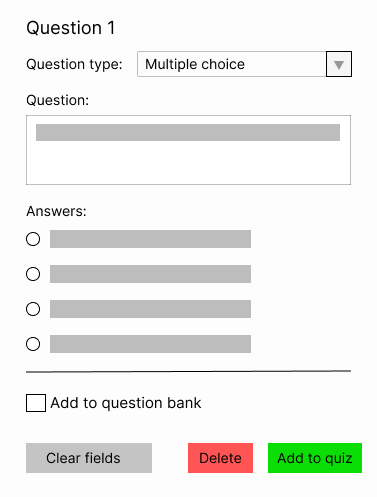
\includegraphics[width=0.9\textwidth]{assessments-quiz-creation}
		\caption{Quiz creation (Instructor's view)}
	\end{minipage}\hfill
	\begin{minipage}{0.45\textwidth}
		\centering
		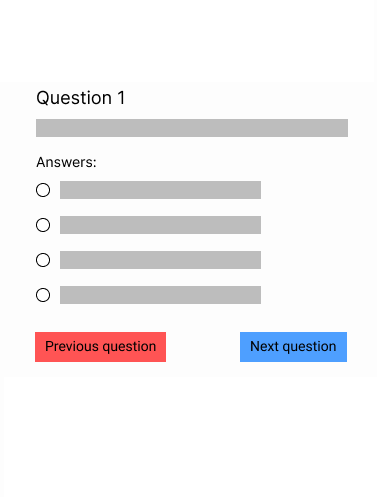
\includegraphics[width=0.9\textwidth]{assessments-quiz-usage}
		\caption{Quiz usage (Student's view)}
	\end{minipage}\hfill
\end{figure}

The core features for polls include being able to:
\begin{itemize}
	\item create/remove a poll
	\item create/remove/edit a poll option
	\item select poll options/s to vote and change your vote
	\item choose between two types of polls to create:
		\begin{itemize}
			\item restricted - can only vote for 1 option
			\item open - can vote for multiple options
		\end{itemize}
\end{itemize}


\subsection{Stakeholders}
\begin{itemize}
	\item Course lecturers
	\item Admins
	\item Students
\end{itemize}

\subsection{Functional Requirements}
The list of functional requirements' priority level will be determined using the MoSCoW method to clearly outline what needs to be implemented throughout the thesis and what the minimum viable product should have. 

The MoSCoW method splits requirements based on 4 categories:
\begin{itemize}
	\item \textcolor{Red}{Must Have}
	\item \textcolor{Blue}{Should Have}
	\item \textcolor{Orange}{Could Have}
	\item \textcolor{Green}{Won't Have}
\end{itemize}

A requirements survey was conducted and completed by me and other Thesis A students to gauge what was the priorities for each requirement. The results for the Assessment feature from the survey and my own ideas were combined to form the following functional requirements:

\subsubsection{Quiz creation}
\begin{enumerate}
	\item Course lecturers can create a quiz \textcolor{Red}{[Must Have]}
	\item Course lecturers can add questions to a quiz \textcolor{Red}{[Must Have]}
	\item Course lecturers can create different types of quiz questions (multiple-choice, short answer, checkboxes) \textcolor{Red}{[Must Have]}
	\item Course lecturers can set up a timer or due date for a quiz \textcolor{Red}{[Must Have]}
	\item Course lecturers can add ``drag and drop" type questions \textcolor{Orange}{[Could Have]}
	\item Course lecturers can add ``connect the pairs" type questions \textcolor{Orange}{[Could Have]}
	\item Course lecturers can add media (audio or  video) into a question as the entire question or as a supplementary material to the question \textcolor{Orange}{[Could Have]}
	\item Course lecturers can create a question bank \textcolor{Blue}{[Should Have]}
	\item Course lecturers can add a question to a question bank \textcolor{Blue}{[Should Have]}
	\item Course lecturers can import a question from a question bank \textcolor{Blue}{[Should Have]}
\end{enumerate}

\subsubsection{Quiz modification/removal}
\begin{enumerate}
	\item Course lecturers can edit/remove a quiz \textcolor{Red}{[Must Have]}
	\item Course lecturers can edit/remove a question \textcolor{Red}{[Must Have]}
	\item Course lecturers can remove a question bank \textcolor{Blue}{[Should Have]}
	\item Course lecturers can remove a question from a question bank \textcolor{Blue}{[Should Have]}
\end{enumerate}

\subsubsection{Quiz usage}
\begin{enumerate}
	\item Students can answer a quiz question \textcolor{Red}{[Must Have]}
	\item Students can edit any of their answers during the quiz \textcolor{Red}{[Must Have]}
	\item Students can submit a quiz attempt \textcolor{Red}{[Must Have]}
	\item Students can manually save their progress at any time \textcolor{Blue}{[Should Have]}
\end{enumerate}

\subsubsection{Poll creation}
\begin{enumerate}
	\item Course lecturers can create different types of polls (can vote either 1 option only or multiple options) \textcolor{Red}{[Must Have]}
	\item Course lecturers can add an option to a poll \textcolor{Red}{[Must Have]}
\end{enumerate}

\subsubsection{Poll modification/closing}
\begin{enumerate}
	\item Course lecturers can edit/remove options \textcolor{Red}{[Must Have]}
	\item Course lecturers can close polls \textcolor{Red}{[Must Have]}
	\item Course lecturers can set a poll closing date \textcolor{Blue}{[Should Have]}
	\item Course lecturers can close a poll but make results viewable \textcolor{Orange}{[Could Have]}
\end{enumerate}

\subsubsection{Poll usage}
\begin{enumerate}
	\item Students can vote for one or multiple options (depending on poll type) \textcolor{Red}{[Must Have]}
	\item Students can add an option (if course lecturer enables the option for it) \textcolor{Orange}{[Could Have]}
\end{enumerate}

\subsubsection{Viewing quiz results and feedback}
\begin{enumerate}
	\item Students can view results against their answers \textcolor{Blue}{[Should Have]}
	\item Students, course lecturers and admins can see how many students selected each answer for a question \textcolor{Blue}{[Should Have]}
	\item Students can view topic or lecture the question derives from \textcolor{Blue}{[Should Have]}
	\item Students can view an explanation of the correct answer if the question is answered incorrectly \textcolor{Orange}{[Could Have]}
\end{enumerate}

\subsubsection{Re-usability}
\begin{enumerate}
	\item Course lecturers can add a question to a general question bank \textcolor{Blue}{[Should Have]}
	\item Course lecturers can import/export quizzes \textcolor{Blue}{[Should Have]}
	\item Course lecturers can import/export questions \textcolor{Blue}{[Should Have]}
\end{enumerate}


\subsection{Non-functional Requirements}
The non-functional requirements used is heavily inspired by the Jakob Nielsen's 10 usability heuristics that's used to evaluate the usability of user interfaces. 

\begin{enumerate}
	\item \textbf{Efficiency} - users are able to perform tasks without taking too many steps
	\item \textbf{Learnability} - new and returning users are able to quickly learn how to use and interact with the feature on the go
	\item \textbf{Performance} - operations within the feature are completed within a timely manner, resulting in a smooth process
	\item \textbf{Consistency} - components, colour themes and formats are consistent across pages 
	\item \textbf{Aesthetic and minimalist design} - the user interface is appealing and simple while providing the expected features
	\item \textbf{Re-usability} - users are able to re-use components and content they've previously made
\end{enumerate}

\subsubsection{Technologies Used}
The technologies that will be used are:
\begin{itemize}
	\item Back-end runtime environment: Node.js
	\item Web application framework: Express.js
	\item Database management system: PostgreSQL
\end{itemize}

\subsubsection{Database}
The use of a relational database will be ideal as it'll be more organised and querying for particular data related to each other will be easier during the implementation of the Assessment feature. 

Potential tables involved would include a Question, Poll, Quiz and User table. 

\subsubsection{Technologies Used}
The technologies that will be used are:
\begin{itemize}
	\item Web application framework: React
	\item Component library for React: Material UI
\end{itemize}

\subsubsection{Feature Breakdown}
Since the React frameworks structures content into re-usable, isolated components, the Assessment feature will need to be broken down into such components. Below are the main components that will likely be implemented during Term 2:
\begin{itemize}
	\item Question
	\item Quiz
	\item Poll Option
	\item Poll
	\item Timer
	\item Question Bank
	\item Quiz Results
	\item Answer Explanation
\end{itemize}


\subsection{Evaluation}
The system will be evaluated based on:
\begin{itemize}
	\item \textbf{Functional requirements} - what was completed, with the satisfactory being all ``Must Haves" and some ``Should Haves"
	\item \textbf{Non-functional requirements} - whether it satisfies the goals of the feature and performs operations in a timely manner
	\item \textbf{Usability tests} - if users can navigate through the feature and be able to complete operations within the feature
\end{itemize}


\newpage
